\chapter{Технологический раздел}
В рамках технологической части были выбраны средства реализации проекта,
описаны программы для создания и запуска базы данных, триггера валидации карты
и
хранимой процедуры проверки покупки, описанных в конструкторской части. Был
описан алгоритм тестирования разработанных триггера и процедуры.

\section{Средства реализации}
В качестве СУБД был выбран Postgresql~\cite{postgres} так как он позволяет
реализовать разработанную структуру данных и ролевую модель, а также
поддерживает реализацию триггеров на добавление и обновление данных.

Для хранения файлов, в частности изображений карт, было выбрано объектное
хранилище Minio~\cite{minio} так как оно позволяет легко и быстро развернуть
хранилище объектов, независимое от файловой и операционной системы.

\section{Создание базы данных}

В качестве языка основного языка для написания проекта был выбран
Python~\cite{python} так как средств языка достаточно для разработки
приложения, есть библиотеки для взаимодействия с Postgresql~\cite{psycorg2} и
Minio~\cite{minio-python}.

\section{Создание базы данных}

На основе разработанной в конструкторском разделе реляционной схемы были
реализованы таблицы пользователей, партий, игроков, карт, типов карт,
изображений, колод и карт в колодах. В программе создания базы данных задаются
первичные и внешние ключи, ограничения уникальности, обязательность полей и
связи между таблицами.

Создание базы данных происходит в два этапа. На первом этапе создаётся схема
базы данных и накладываются ограничения целостности. Для этого используются
миграции Alembic~\cite{alembic}, которые формируют и последовательно применяют
SQL-команды создания и изменения таблиц. Скрипт представлен в приложении А в
листинге~\ref{lst:alembic}.

На втором этапе база данных заполняется начальными данными: типами карт,
изображениями и набором игровых карт. Этап заполнения базы данных представлен в
листинге~\ref{lst:fill_db}.

Интерфейс доступа к базе данных реализован через репозитории пользователей,
карт, типов карт и партий. Репозитории используют сессии SQLAlchemy,
создаваемые фабрикой \texttt{SessionFactory}, поэтому прикладная логика
обращается к базе данных через методы предметного уровня, а не через
SQL-запросы напрямую.

\section{Роли и их права}
В конструкторской части были выделены следующие пять ролей:
\begin{itemize}
	\item пользователь (гость);
	\item авторизованный пользователь;
	\item игрок;
	\item модератор;
	\item мастер.
\end{itemize}

Кроме стандартных прав на уровне ролей, для дополнительной защиты данных
использовалась фильтрация строк PostgreSQL \texttt{postgres-rls}, которая
ограничивает доступ к записям в таблицах на уровне строк.

Код для создания ролей и определения прав доступа представлен в приложении А в
листингах~\ref{lst:user-role}~---~\ref{lst:master-role}.

\section{Триггер валидации карты}

Для обеспечения целостности данных был разработан триггер, который при каждом
вставлении или обновлении записи в таблице \texttt{cards} проверяет
соответствие характеристик карты установленным ограничениям. Если одно из
условий не выполняется, триггер прерывает операцию и откатывает изменение.
Код разработанного триггера представлен в приложении А, в
листинге~\ref{lst:card_check_trigger}.

\section{Процедура проверки покупки}

Для проверки покупки карты была реализована хранимая процедура, которая
проверяет доступность карты, текущее эхо игрока и бизнес-правила перед
совершением покупки. Если объём эхо меньше стоимости карты, процедура
генерирует исключение, и операция покупки не выполняется.
Код хранимой процедуры представлен в приложении А, в
листинге~\ref{lst:card_buy_procedure}.

\section{Redis (кэширование)}

Для повышения производительности системы при работе с каталогом карт
используется Redis~\cite{redis}, его применение позволяет сократить количество
обращений к базе данных.

В кэше сохраняются готовые JSON-ответы для эндпоинтов, предназначенных только
для просмотра данных каталога карт. При поступлении запроса система сначала
проверяет наличие соответствующих данных в Redis. Если данные найдены, ответ
формируется непосредственно из кэша, в противном
случае информация извлекается из базы данных, преобразуется в
JSON-представление и сохраняется в Redis для последующих запросов.

Для обеспечения актуальности данных каждой записи в кэше назначается
ограниченное время жизни (TTL, Time To Live). После истечения этого времени
запись автоматически удаляется из Redis и при следующем обращении формируется
заново на основе данных из базы данных.

При добавлении, изменении или удалении карты записи кэша, связанные с каталогом
карт, принудительно удаляются.

\section{Пользовательский интерфейс}

В качестве пользовательского интерфейса было разработано веб-приложение с
игрой, предоставляющее описанную в аналитической части функциональность.
Приложение разделено на основные компоненты, представляющие различные этапы
взаимодействия пользователя с системой: авторизация, просмотр каталога карт,
редактирование колод и процесс игровой сессии. Описание компонентов
пользовательского интерфейса представлено в UML формате на
рисунке~\ref{img:ui-uml}.

\begin{figure}[H]
	\centering
	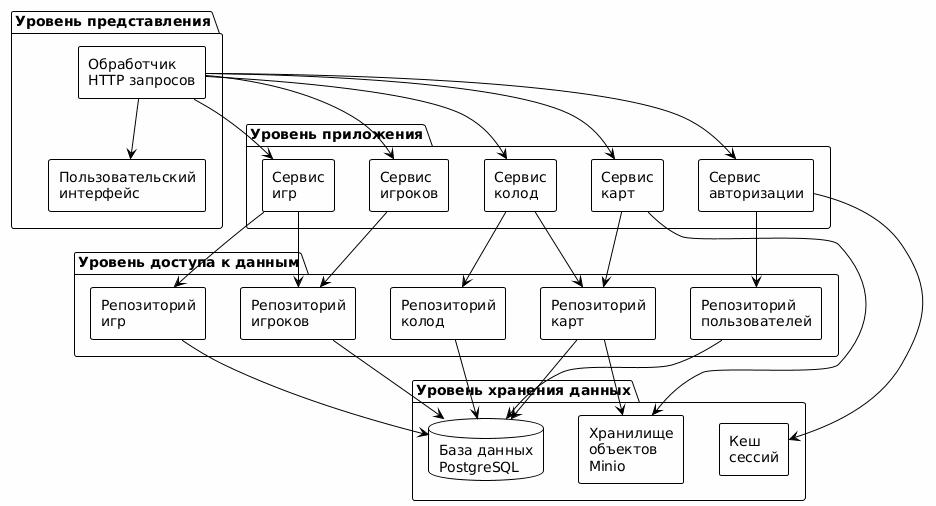
\includegraphics[width=0.9\linewidth]{../img/ui-uml}
	\caption{Диаграмма компонентов пользовательского интерфейса}
	\label{img:ui-uml}
\end{figure}

\section{Тестирование}

\subsection{Тестирование приложения}

Модульное тестирование приложения проводилось с помощью фреймворка
\texttt{pytest}~\cite{pytest} и стандартной библиотеки
\texttt{unittest.mock} для изоляции тестируемых компонентов.

Тестами были покрыты модули игровой логики, логики карт, управления
состоянием партии, сервиса колод и контроля доступа.

Покрытие кода составило 84\%.

\subsection{Тестирование триггера валидации карты}

Тестирование триггера проводилось с помощью тестов на языке Python.
Были выделены следующие классы эквивалентности:

\begin{itemize}
	\item корректная карта (все поля в допустимых пределах);
	\item карта с нулевой стоимостью (\texttt{cost} = 0);
	\item карта со стоимостью выше максимума (\texttt{cost} > 7);
	\item карта с нулевой силой (\texttt{power} = 0);
	\item карта типа \texttt{buff\_*} с силой выше 2 (\texttt{power} > 2);
	\item карта с \texttt{cool\_points} ниже минимума (< $-1$);
	\item карта с \texttt{cool\_points} выше максимума (> 5);
	\item карта без типа (\texttt{card\_type\_id} = NULL);
	\item карта типа \texttt{buff\_*} с пустым полем \texttt{creature};
	\item карта типа \texttt{buff\_*} с непустым полем \texttt{creature}.
\end{itemize}

Каждый класс эквивалентности был протестирован на операциях вставки
и обновления. Общий алгоритм тестирования триггера имел следующий вид:

\begin{enumerate}
	\item Создание тестовых данных в базе данных (тип карты, изображение).
	\item Цикл по всем тестам:
	      \begin{enumerate}
		      \item вставка записи карты с тестовыми данными;
		      \item если тест позитивный:
		            \begin{itemize}
			            \item проверка, что триггер не вызвал
			                  ошибку;
			            \item проверка, что запись успешно
			                  добавлена в таблицу;
		            \end{itemize}
		      \item иначе:
		            \begin{itemize}
			            \item проверка, что триггер вызвал ошибку;
			            \item проверка, что запись не добавлена в
			                  базу данных;
		            \end{itemize}
		      \item очистка таблицы карт.
	      \end{enumerate}
	\item Цикл по всем тестам:
	      \begin{enumerate}
		      \item создание корректной записи карты;
		      \item обновление записи согласно тестовым данным;
		      \item если тест позитивный:
		            \begin{itemize}
			            \item проверка, что триггер не вызвал
			                  ошибку;
			            \item проверка, что запись успешно
			                  изменена;
		            \end{itemize}
		      \item иначе:
		            \begin{itemize}
			            \item проверка, что триггер вызвал ошибку;
			            \item проверка, что запись не изменена.
		            \end{itemize}
	      \end{enumerate}
\end{enumerate}

\subsection{Тестирование процедуры проверки покупки}

Тестирование хранимой процедуры проводилось с помощью тестов на языке Python.
Были выделены следующие классы эквивалентности:

\begin{itemize}
	\item корректная покупка при достаточном количестве эхо;
	\item покупка при недостаточном количестве эхо;
	\item покупка несуществующей карты;
	\item покупка карты, которой нет в каталоге.
\end{itemize}

Общий алгоритм тестирования процедуры имел следующий вид:

\begin{enumerate}
	\item Создание тестовых данных: игрока с заданным количеством эхо и
	      карты с заданной стоимостью.
	\item Вызов процедуры с тестовыми параметрами.
	\item Если тест позитивный:
	      \begin{itemize}
		      \item проверка, что процедура не вызвала исключение;
		      \item проверка, что стоимость карты вычтена из баланса
		            эхо
		            игрока;
		      \item проверка, что карта добавлена в колоду игрока.
	      \end{itemize}
	\item Иначе:
	      \begin{itemize}
		      \item проверка, что процедура вызвала исключение;
		      \item проверка, что баланс эхо игрока не изменился;
		      \item проверка, что карта не добавлена в колоду игрока.
	      \end{itemize}
\end{enumerate}

\section*{Вывод}
В результате технологической части были выбраны средства реализации работы,
созданы
база данных, роли, триггер и хранимая процедура. Также было разработано и
протестировано приложение для игры.